\documentclass[11pt]{article}

\usepackage{nmrdoc}
\usepackage{listings}
\usepackage[utf8]{inputenc}

\lstset{
  basicstyle=\ttfamily\small,
  breaklines=true,
  columns=fullflexible,
  keepspaces=true,
  frame=single,
  xleftmargin=1em,
  xrightmargin=1em
}

\newcommand{\code}[1]{\texttt{#1}}
\newcommand{\tensor}[1]{\boldsymbol{#1}}

\emergencystretch=3em
\setlength{\parindent}{0pt}
\setlength{\parskip}{0.5em}
\AtBeginDocument{\raggedright}

\begin{document}
\NmrTitle{Object Model and Runtime Architecture of the NMR Shielding Extractor}
\tableofcontents
\clearpage

\section{Authority and scope}

This document describes the object model and runtime architecture used by the
NMR chemical-shielding extractor. The design documents
\code{OBJECT\_MODEL.md}, \code{PATTERNS.md}, and
\code{spec/CONSTITUTION.md} state the intent: typed objects, no runtime string
dispatch for chemical identity, geometry separated from invariant protein
identity, and full rank-2 tensor output. The source is the authority for the
exact type names, ownership, and call order.

The code read for this document is:
\code{Protein}, \code{ProteinConformation}, \code{ProteinTopology},
\code{ConformationResult}, \code{DenseBuffer}, \code{OperationRunner},
\code{OperationLog}, \code{Session}, \code{Trajectory},
\code{TrajectoryProtein}, and \code{RunConfiguration}, with the adjacent
headers that define the actual per-atom records:
\code{ConformationAtom}, \code{TrajectoryAtom}, \code{TrajectoryResult},
\code{Atom}, \code{Residue}, \code{Bond}, \code{Ring}, and
\code{LegacyAmberTopology}.

The reader should keep one boundary in mind:
\[
  \text{Protein identity/topology}
  \quad \ne \quad
  \text{conformation geometry}
  \quad \ne \quad
  \text{trajectory history}.
\]
The code enforces this with separate objects and separate ownership.

\section{The system in one page}

The architecture is shaped around one separation: a protein's identity and topology ---
its atoms, residues, bonds, and rings --- are fixed once built, while everything that
depends on coordinates is not. Identity is held in one invariant object; a conformation
holds a coordinate set and the results computed from it; a trajectory holds the history
across frames. Ownership, call order, and buffer placement follow from keeping these
three apart.

The extractor is a one-way accumulation system. A loader builds a
\code{Protein}; a conformation supplies one coordinate set for that protein;
\code{OperationRunner::Run} attaches named \code{ConformationResult}
singletons to that conformation in dependency order; trajectory mode repeats
that conformation-level run for streamed frames and lets
\code{TrajectoryResult} objects accumulate over the frame sequence.

\subsection{Primary objects}

\begin{description}
\item[\code{Protein}] The invariant protein. It owns atoms, residues,
the topology object, force-field charge table, build context, and any permanent
conformations. It holds no atom coordinates and no computed shielding fields.

\item[\code{LegacyAmberTopology}] The concrete topology attached to
\code{Protein}. It owns \code{CovalentTopology}, \code{RingTopology},
force-field invariant fields captured at the loader boundary, and the
per-atom typed chemistry substrate \code{AtomSemanticTable}.

\item[\code{ProteinConformation}] One coordinate set for a protein. It owns
the position vector, the parallel \code{ConformationAtom} vector, derived
geometry caches such as ring geometries and bond midpoints, and the attached
\code{ConformationResult} map.

\item[\code{ConformationAtom}] The per-atom computed-data record for one
conformation. It stores position and the typed fields written by calculators:
charges, neighbour records, tensors, spherical decompositions, solvent fields,
DFT tensors, and feature-side values. It does not duplicate element or residue
identity and does not own topology; bond and ring references appear only inside
computed neighbourhood records.

\item[\code{ConformationResult}] The named operation object for
conformation-scope computation. It declares a name, type-index dependencies,
and optional feature writing. Subclasses own the physics query surface and write
their results into \code{ConformationAtom} fields or into result-owned state.

\item[\code{TrajectoryProtein}] The trajectory-scope protein. It wraps the
owned \code{Protein}, seats the first dispatched frame (trajectory frame 0, or
\code{window\_start} when windowed) as a permanent
\code{MDFrameConformation}, allocates one \code{TrajectoryAtom} per protein
atom, owns attached \code{TrajectoryResult}s, and receives dense buffers at
finalization.

\item[\code{TrajectoryAtom}] The per-atom trajectory record. It holds named
Welford state substructs and an atom-scope \code{RecordBag<AtomEvent>}. It
does not hold position or identity.

\item[\code{Trajectory}] The run process and post-run record. It owns source
paths, frame times, frame indices, the single-slot \code{TrajectoryEnv}, the
run-scope \code{RecordBag<SelectionRecord>}, and the
\code{GromacsFrameHandler} while the run is active.

\item[\code{RunConfiguration}] A typed run shape: per-frame
\code{RunOptions}, deferred \code{TrajectoryResult} factories, required
per-frame \code{ConformationResult} types, AIMNet2 requirement, and stride.
\end{description}

\subsection{Static and trajectory flows}

The static conformation flow is short:

\begin{lstlisting}
loader builds Protein
Protein::FinalizeConstruction(positions)
Protein::AddConformation / AddCrystalConformation / AddPrediction / AddMDFrame
OperationRunner::Run(conf, RunOptions)
ConformationResult::WriteAllFeatures(conf, output_dir)
\end{lstlisting}

The trajectory flow keeps the same per-frame computation and adds one outer
streaming layer:

\begin{lstlisting}
TrajectoryProtein::BuildFromTrajectory(dir)
Trajectory::Run(tp, config, session, extras, output_dir)
  open GromacsFrameHandler
  optionally skip to window_start
  read seed frame
  tp.Seed(seed_positions, time_ps)
  attach TrajectoryResults from RunConfiguration
  validate dependencies and Session resources
  build per-frame RunOptions
  emit invariant atom/topology sidecars if output_dir is set
  seed frame:
    update TrajectoryEnv and frame RunOptions
    conf0 = tp.MutableCanonicalConformation_()
    OperationRunner::Run(conf0, opts)
    tp.DispatchCompute(conf0, traj, frame_index, time)
  each later dispatched frame:
    stop at window_start + window_len when windowed
    skip/read according to stride
    update TrajectoryEnv and frame RunOptions
    conf = tp.TickConformation(positions)
    OperationRunner::Run(*conf, opts)
    tp.DispatchCompute(*conf, traj, frame_index, time)
  tp.FinalizeAllResults(traj)
\end{lstlisting}

The first dispatched frame is permanent and is an
\code{MDFrameConformation}; it is trajectory frame 0 for a full run and
\code{window\_start} for a windowed run. Later streamed frames are
free-standing base \code{ProteinConformation} instances returned by
\code{TrajectoryProtein::TickConformation}; they point at the wrapped
\code{Protein} for topology and die at the end of the loop iteration. There
is no separate per-frame geometry class.

\section{Diagrams}

The diagrams in this section were rendered from Mermaid sources with
\code{mmdc} and the Puppeteer configuration in
\code{doc/calculators/.puppeteerrc.json}. They are included as PDFs so the
compiled document is self-contained.

\begin{figure}[p]
\centering
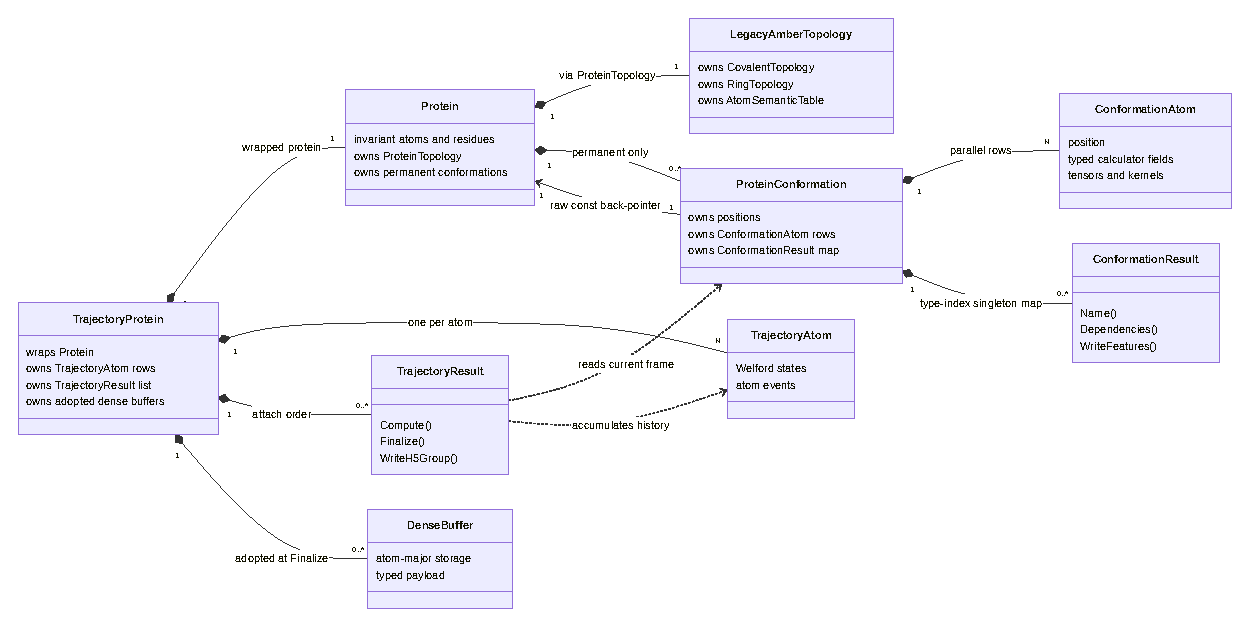
\includegraphics[width=\textwidth,height=0.76\textheight,keepaspectratio]{architecture_object_model.pdf}
\caption{Object-model ownership and dependency relationships. Permanent
conformations are owned by \code{Protein}; later streamed frames are temporary
\code{ProteinConformation} objects owned by the trajectory loop.}
\label{fig:object-model}
\end{figure}

\begin{figure}[p]
\centering
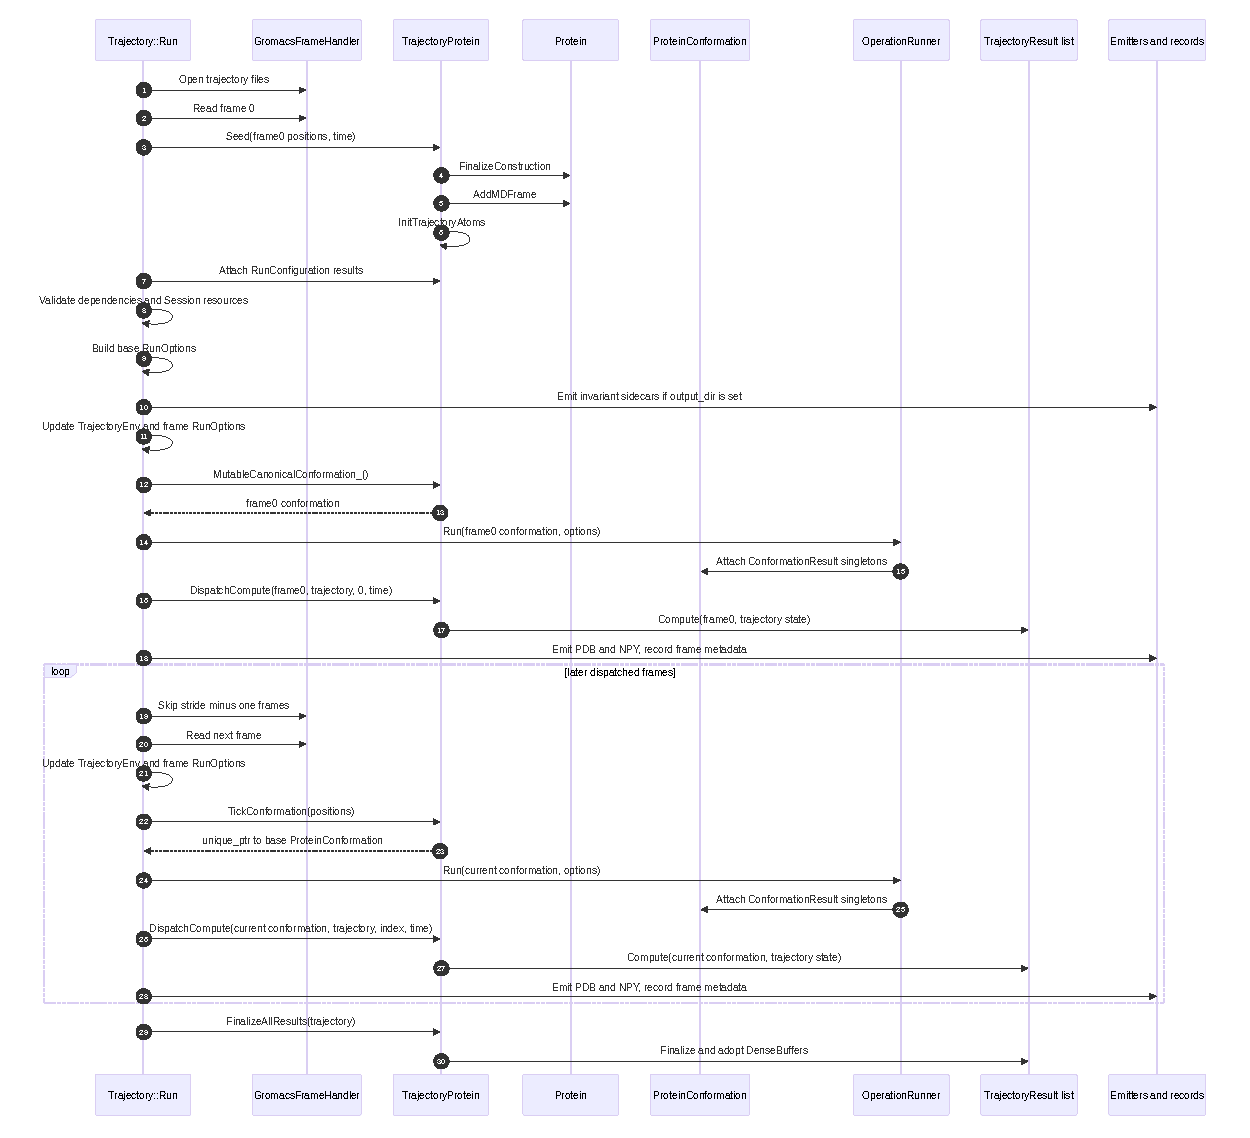
\includegraphics[width=\textwidth,height=0.82\textheight,keepaspectratio]{architecture_per_frame_flow.pdf}
\caption{Per-frame trajectory call flow, showing the permanent frame-zero
conformation and the temporary later-frame conformations.}
\label{fig:per-frame-flow}
\end{figure}

\clearpage

\section{Protein identity and topology}

\code{Protein} is non-copyable and non-movable. The reason is concrete:
\code{ProteinConformation} stores a raw \code{const Protein*} back-pointer, and
deleting move construction prevents that pointer from being invalidated by a
moved parent.

\code{Protein} owns these member groups:

\begin{lstlisting}
std::vector<std::unique_ptr<Atom>> atoms_;
std::vector<Residue> residues_;
std::unique_ptr<ProteinTopology> protein_topology_;
std::unique_ptr<ForceFieldChargeTable> force_field_charges_;
std::unique_ptr<ProteinBuildContext> build_context_;
std::vector<std::unique_ptr<ProteinConformation>> conformations_;
\end{lstlisting}

The direct storage point for bonds and rings is not \code{Protein}. In current
code \code{Protein} delegates \code{BondAt}, \code{Bonds},
\code{RingAt}, \code{Rings}, and the saturated-ring accessors through
\code{LegacyAmberTopology}. \code{Protein::BondCount()} and
\code{Protein::RingCount()} return zero before topology exists; the bond and
ring element/list accessors require the topology and abort if it is missing.

\subsection{Atoms, residues, bonds, and rings}

\code{Atom} is a flat identity record:
\code{element}, display/serialization name \code{pdb\_atom\_name},
\code{residue\_index}, \code{bond\_indices}, and
\code{parent\_atom\_index}. The methods \code{CovalentRadius},
\code{Electronegativity}, \code{IsHBondDonorElement}, and
\code{IsHBondAcceptorElement} answer element-derived questions. There is no
atom subclass hierarchy.

\code{Residue} stores amino-acid identity, sequence address, atom indices,
protonation variant, terminal-state metadata, cached backbone slots
\code{N}, \code{CA}, \code{C}, \code{O}, \code{H}, \code{HA},
\code{CB}, and up to four \code{ChiAtoms} records. It answers residue-level
questions through methods such as \code{IsAromatic}, \code{IsTitratable},
\code{HasAmideH}, and \code{ChiAngleCount}. Backbone adjacency is not inferred
from chain labels or sequence numbers; \code{Protein::BackbonePredecessor},
\code{BackboneSuccessor}, and \code{BackboneConnected} walk the peptide bond
graph.

\code{Bond} stores atom endpoints, \code{BondOrder}, \code{BondCategory}, and
\code{is\_rotatable}. Its geometry methods take a position vector because
midpoint, length, and direction depend on a conformation. The topology stays
invariant; geometry is computed from the coordinate set supplied at the call
site.

\code{Ring} is a virtual type hierarchy. A ring stores vertex atom indices,
\code{RingTypeIndex}, parent residue, parent residue number, and fused partner.
The type-specific physics is virtual: \code{Intensity},
\code{LiteratureIntensity}, \code{JohnsonBoveyLobeOffset},
\code{NitrogenCount}, \code{Aromaticity}, \code{RingAtomCount}, and
\code{TypeName}. The current classes include \code{PheBenzeneRing},
\code{TyrPhenolRing}, \code{TrpBenzeneRing}, \code{TrpPyrroleRing},
\code{HisImidazoleRing}, \code{HidImidazoleRing}, \code{HieImidazoleRing},
\code{IndolePerimeterRing}, and the saturated
\code{ProPyrrolidineRing}. The aromatic-type boundary is
\code{kAromaticRingTypeCount = 8}; \code{ProPyrrolidine} is the first
saturated type.

\subsection{Topology construction order}

Every loader must call \code{Protein::FinalizeConstruction} after adding
atoms and residues and before adding any conformation. In source order, the
method does the following:

\begin{lstlisting}
ResolveResidueTerminalStates()
CacheResidueBackboneIndices()
ResolveProtonationStates(nullptr)
CovalentTopology::Resolve(atoms_, residues_, positions, bond_tolerance)
if disulfide authority exists:
  bonds->OverrideDisulfides(authority_pairs)
ResolveProtonationStates(bonds.get())
copy bond indices and hydrogen parents back onto Atom
run post-protonation NamingApplicator pass
ComposeAtomSemantic(atoms_, residues_, *bonds)
RingTopology::ConstructFromSubstrate(residues_, atom_semantic, *bonds)
bonds->TagAromaticBonds(rings->Aromatic())
construct LegacyAmberTopology(...)
CacheResidueBackboneIndices_Typed()
\end{lstlisting}

This order matters. The first backbone cache is a loader-boundary string pass;
the final cache is substrate-driven and overwrites the earlier slots. Ring
construction happens after protonation and semantic composition, and aromatic
bond tagging is an overlay after rings exist. \code{DetectAromaticRings} is no
longer part of the path.

\section{Conformation scope}

\code{ProteinConformation} is the geometry object. Its constructor takes a
borrowed \code{Protein*}, a \code{std::vector<Vec3>} of positions, and an
optional description. It moves the positions into \code{positions\_}, then
constructs \code{atoms\_} as one \code{ConformationAtom} per position.
The \code{ConformationAtom} constructor is private and
\code{ProteinConformation} is its friend, so loose per-conformation atom
records cannot be created outside the owning conformation.

The conformation stores:

\begin{itemize}
\item \code{positions\_}, returned by \code{Positions};
\item \code{atoms\_}, the parallel \code{ConformationAtom} vector whose
position copy is read by \code{PositionAt};
\item \code{results\_}, an unordered map keyed by \code{std::type\_index}
and owning \code{ConformationResult} pointers;
\item ring geometry, ring pair records, bond lengths, bond directions,
bond midpoints, bounding box, center of geometry, radius of gyration, and
pre-built maps by ring type, bond category, and residue type;
\item \code{geometry\_choices}, the recorded geometric decisions made during
\code{Compute}.
\end{itemize}

The geometry boundary is therefore explicit. Static identity is read through
\code{conf.ProteinRef().AtomAt(i)} and topology through
\code{conf.ProteinRef().LegacyAmber()}. Coordinate and computed data are read
from \code{conf.PositionAt(i)} and \code{conf.AtomAt(i)}.

\subsection{Conformation subclasses}

\code{ProteinConformation} is not abstract. It is the complete working
geometry object. The subclasses only add provenance:

\begin{description}
\item[\code{CrystalConformation}] resolution, R factor, temperature, PDB ID.
\item[\code{PredictionConformation}] prediction method and confidence.
\item[\code{MDFrameConformation}] walker, time in ps, Boltzmann weight, RMSD,
and radius of gyration.
\item[\code{DerivedConformation}] derivation description.
\end{description}

\code{Protein::AddDerived} does not store the parent argument; the current
code uses it only to select the factory signature.

\subsection{ConformationResult attachment}

\code{ConformationResult} is the base class for computed conformation-scope
results:

\begin{lstlisting}
virtual std::string Name() const = 0;
virtual std::vector<std::type_index> Dependencies() const = 0;
virtual int WriteFeatures(const ProteinConformation&, const std::string&) const;
\end{lstlisting}

\code{ProteinConformation::AttachResult} checks three facts:

\begin{itemize}
\item the pointer is not null;
\item no result of the same dynamic type is already attached;
\item every declared dependency is already present in \code{results\_}.
\end{itemize}

If the null check fails, \code{AttachResult} returns false. Duplicate or
missing-dependency failures are rejected with a warning. If the checks pass,
the result is stored under \code{typeid(*result)}. The
\code{Result<T>} accessor returns the typed result and aborts if it is absent;
\code{HasResult<T>} is the non-aborting presence check. The code therefore
uses typed access, not string dispatch on result names.

Computation happens before attachment, in each subclass's static
\code{Compute} factory. Attachment validates the singleton and dependency
contract; it does not run the calculator.

\subsection{ConformationAtom as the computed-data row}

\code{ConformationAtom} is the per-atom computed-data row for one
conformation. Its immutable field is the constructor-set \code{position\_}.
Everything else is typed, public calculator output. Important groups include:

\begin{itemize}
\item enrichment fields: \code{role}, \code{hybridisation},
\code{is\_backbone}, \code{is\_amide\_H}, \code{is\_hbond\_donor}, and
related booleans;
\item force-field and MOPAC charges, PB radii, orbital populations, Wiberg
neighbours;
\item \code{spatial\_neighbours}, \code{ring\_neighbours}, and
\code{bond\_neighbours};
\item ring-current totals, McConnell totals, Coulomb fields, MOPAC Coulomb
fields, APBS fields, H-bond fields, ring-based shielding kernels, graph
fields, ORCA DFT tensors, tripeptide and Larsen tensors, AIMNet2 tensors,
planar geometry, SASA, water fields, hydration geometry, EEQ charges, and
prediction fields.
\end{itemize}

The per-source structured records are real types:
\code{RingNeighbourhood}, \code{BondNeighbourhood}, \code{AtomNeighbour}, and
\code{MopacBondNeighbour}. \code{RingNeighbourhood} stores the ring identity,
ring-frame geometry, and per-ring calculator tensors. \code{BondNeighbourhood}
stores bond identity, bond category, midpoint geometry, dipolar tensor, its
spherical decomposition, and the McConnell scalar.

\section{Tensor representation}

The tensor output is preserved end to end. \code{Types.h} defines
\code{Vec3} and \code{Mat3} as Eigen types and \code{SphericalTensor} as:

\begin{lstlisting}
double T0;
std::array<double, 3> T1;
std::array<double, 5> T2;
\end{lstlisting}

\code{SphericalTensor::Decompose} maps a real \(3\times3\) tensor into
irreducible components: isotropic \(T_0\), antisymmetric pseudovector \(T_1\),
and symmetric traceless \(T_2\) in the code's real isometric basis.
\code{PackFull9} emits the order
\[
  [T_0, T_{1x}, T_{1y}, T_{1z},
    T_{2,-2}, T_{2,-1}, T_{2,0}, T_{2,+1}, T_{2,+2}].
\]
\code{PackT2} exists for sources that are structurally pure \(T_2\).
\code{T2CosineWith} is a method on \code{SphericalTensor}; this is another
example of an object answering a physics question about itself rather than
shipping its arrays to a string-selected helper.

The wide \code{ConformationAtom} row contains both matrices and decomposed
tensors when a calculator produces both. Examples include
\code{total\_G\_tensor} with \code{total\_G\_spherical},
\code{coulomb\_EFG\_total} with
\code{coulomb\_EFG\_total\_spherical}, \code{apbs\_efg} with
\code{apbs\_efg\_spherical}, ORCA dia/para/total matrix+spherical pairs,
and Larsen tensor+spherical pairs. Classical kernel totals such as
\code{bs\_shielding\_contribution},
\code{mc\_shielding\_contribution}, and
\code{coulomb\_shielding\_contribution} are stored as
\code{SphericalTensor}; this model does not scalarize them at storage time.

\section{OperationRunner}

\code{OperationRunner} is the one place that runs the ordered conformation-level
sequence, and it holds no state of its own. It takes a mutable \code{ProteinConformation}
and a \code{RunOptions} value, computes the result objects in order, and attaches each to
the conformation. A result is self-contained: a subclass declares its name and its
type-index dependencies, holds the query surface and the typed output for its one
computation, and is retrieved by its type, not by a string name. A calculator that
depends on another result reads it from the conformation by type; there is no shared
property store.

The current \code{RunOptions} surface is larger than the early design notes:
charge source and net charge; skip flags for DSSP, MOPAC, APBS, and vacuum
Coulomb; an AIMNet2 model pointer; GROMACS frame energy; solvent; bonded
parameters; per-frame velocities and box matrix; ORCA NMR path; tripeptide DFT
table; and Larsen H-bond grid.

The exact \code{OperationRunner::Run} order is:

\begin{lstlisting}
GeometryResult
SpatialIndexResult
EnrichmentResult
PlanarGeometryResult        // soft attach; logs and continues on null
DsspResult                  // unless skip_dssp; soft external-tool policy
ChargeAssignmentResult      // if charge_source exists

if ChargeAssignmentResult attached:
  MopacResult               // unless skip_mopac; soft failure
  ApbsFieldResult           // unless skip_apbs; soft failure

BiotSavartResult
HaighMallionResult
McConnellResult
RingSusceptibilityResult
PiQuadrupoleResult
DispersionResult
CoulombResult               // if charges and !skip_coulomb
MopacCoulombResult          // if MopacResult attached
MopacMcConnellResult        // if MopacResult attached
HBondResult                 // if DsspResult attached
SasaResult
EeqResult
AIMNet2Result
AIMNet2ChargeResponseGradientResult
WaterFieldResult
HydrationShellResult
HydrationGeometryResult
GromacsFramePullResult
GromacsEnergyResult
BondedEnergyResult
TripeptideBackboneShieldingResult
TripeptideNeighborShieldingResult
LarsenHBondShieldingResult
OrcaShieldingResult         // optional; non-empty path failing is fatal
\end{lstlisting}

Some entries are hard requirements once requested. AIMNet2, explicit solvent
calculators, GROMACS frame pull, energy, bonded energy, and the tripeptide and
Larsen resources use \code{TimedAttach} or \code{Attach} failure to stop the
run. DSSP, MOPAC, APBS, and planar geometry are allowed to be absent for
specific input/resource failures and leave their result absent rather than
faking data.

\code{RunMutantComparison} runs \code{Run} on WT and ALA conformations and, if
both have \code{OrcaShieldingResult}, computes \code{MutationDeltaResult}
against the mutant and attaches the delta to the WT conformation. The mutant
is an input to the computation, not the owner of the delta result.

\section{Trajectory runtime}

\code{Trajectory::Run} drives the trajectory run. It is the only code path
with mutable access to frame-zero conformation through the private
\code{TrajectoryProtein::MutableCanonicalConformation\_} friend hook. Public
\code{TrajectoryProtein} exposes \code{ProteinRef} and
\code{CanonicalConformation} as const, so \code{TrajectoryResult} subclasses
cannot mutate the invariant protein or the per-instant conformation buffer
through \code{TrajectoryProtein}.

\subsection{Run phases}

The eight phases in \code{Trajectory::Run} are:

\begin{enumerate}
\item Open \code{GromacsFrameHandler}.
\item Read the seed frame and call \code{TrajectoryProtein::Seed}.
\item Attach \code{TrajectoryResult}s from \code{RunConfiguration} factories,
then caller extras.
\item Validate dependencies and session resources.
\item Build the base \code{RunOptions} template, then emit invariant
atom/topology sidecars if an output directory is set.
\item Run the seed frame through \code{OperationRunner}, dispatch trajectory
results, emit per-frame PDB/NPY, and record frame metadata.
\item For each later dispatched frame: skip according to stride, read, update
\code{TrajectoryEnv}, create a tick conformation, run
\code{OperationRunner}, dispatch trajectory results, emit, and record.
\item Finalize all trajectory results, mark complete, and release the handler.
\end{enumerate}

Dependency validation is split deliberately. \code{TrajectoryProtein::AttachResult}
checks only singleton-per-type. Phase 4 checks each
\code{TrajectoryResult::Dependencies()} entry against either an attached
trajectory result or the \code{RunConfiguration} set of required
per-frame \code{ConformationResult} types. AIMNet2 is validated as a
\code{Session} resource if the configuration requires it.

\subsection{Frame environment}

\code{TrajectoryEnv} is a single-slot frame environment. It stores solvent,
current energy pointer, frame index, frame time, velocities, and box matrix.
\code{Trajectory::Run} overwrites it before each dispatched frame. Results
that need history copy what they need into their own state during
\code{Compute}; \code{TrajectoryEnv} is not a history buffer.

\section{Buffer management}

The system's buffer discipline is constructor allocation with scoped ownership: a buffer
is allocated by the object whose lifetime defines its validity, when that object is
built. The sizes are known at that point --- the atom count, the per-atom stride --- so
nothing is grown or attached afterward. A conformation sizes its atom rows from the
position vector it receives; a \code{TrajectoryProtein} sizes its per-atom records once
the seed frame fixes the atom count; on creation, a \code{DenseBuffer} holds the atom
count and the stride per atom. The lifetime defines the validity; there is no
register/release step and no detach.

\subsection{Conformation buffers}

\code{ProteinConformation} owns \code{positions\_} and the parallel
\code{atoms\_} vector. Both are sized in the constructor from the input
position vector. A \code{ConformationAtom} contains its own position copy as
\code{position\_}; \code{PositionAt(i)} returns that value, while
\code{Positions()} returns the source vector. Calculators write typed fields
onto the \code{ConformationAtom} row.

\code{ConformationResult} objects are owned by the conformation under
\code{std::unique\_ptr}. There is no separate property-store framework.
The older design idea of a typed store interface does not exist in current
code; result \code{Compute} methods write the named fields directly.

\subsection{TrajectoryAtom buffers}

\code{TrajectoryProtein::Seed} finalizes the wrapped protein, seats the first
dispatched frame, and then calls \code{InitTrajectoryAtoms}. That method
clears and reserves the vector to \code{protein\_->AtomCount()} and constructs one
\code{TrajectoryAtom} per atom. \code{TrajectoryAtom} has a private default
constructor and \code{TrajectoryProtein} is its friend, so the trajectory atom
buffer is only created by the owning \code{TrajectoryProtein}.

The current \code{TrajectoryAtom} stores named Welford state substructs:
\code{bs\_welford}, \code{hm\_welford}, \code{mc\_welford},
\code{eeq\_welford}, \code{sasa\_welford},
\code{hbond\_count\_welford}, \code{water\_field\_welford},
\code{hydration\_geometry\_welford},
\code{hydration\_shell\_welford},
\code{aimnet2\_charge\_response\_gradient\_welford}, and
\code{mopac\_charge\_welford}. Each substruct has one writer trajectory
result. The atom also owns \code{RecordBag<AtomEvent> events}.

\subsection{DenseBuffer}

\code{DenseBuffer<T>} is the finalize-only time-series and lag buffer. It is
constructed with \code{atom\_count} and \code{stride\_per\_atom}. Its storage is
a single \code{std::vector<T>} of length
\(atom\_count \times stride\_per\_atom\), laid out atom-major:

\begin{lstlisting}
storage[atom_idx * stride_per_atom + offset]
\end{lstlisting}

The result that needs the buffer usually owns it while frames are being
processed. At \code{Finalize}, it transfers ownership to
\code{TrajectoryProtein::AdoptDenseBuffer<T>}, keyed by the owning result's
\code{std::type\_index}. \code{GetDenseBuffer<T>} returns null if the owner key
is absent or if the stored element type differs. This keeps mixed buffer
payloads behind \code{DenseBufferBase} without losing typed access at use
sites.

H5 writers flatten \code{DenseBuffer} content by explicit component access
rather than by reinterpreting raw memory. This is important for Eigen-backed
types and for \code{SphericalTensor}; layout in memory is not the serialization
contract.

\section{RunConfiguration}

\code{RunConfiguration} is a typed named run shape. A shape holds:
\code{name\_}, \code{per\_frame\_opts\_}, deferred trajectory-result factories,
\code{required\_conf\_result\_types\_}, \code{requires\_aimnet2\_}, and
\code{stride\_}. A deferred factory is a callable that takes a const
\code{TrajectoryProtein\&} and returns a
\code{std::unique\_ptr<TrajectoryResult>}.
Factories are deferred because trajectory results size their buffers after
\code{TrajectoryProtein::Seed}, when atom, bond, and ring counts are known.

The code currently exposes two named shapes:

\begin{description}
\item[\code{PerFrameExtractionSet}] Production canonical trajectory shape.
It skips MOPAC and vacuum Coulomb, keeps APBS and DSSP on, requires AIMNet2,
requires the full per-frame conformation stack listed in
\code{RunConfiguration.cpp}, and attaches the Welford, time-series, solvent,
dynamics, geometry, energy, dihedral, ring, and selection trajectory results.

\item[\code{FullFatFrameExtraction}] Starts from \code{PerFrameExtractionSet},
sets \code{skip\_mopac=false} and \code{skip\_coulomb=false}, and appends the
MOPAC-family trajectory results: MOPAC charge Welford, MOPAC bond-order
Welford, MOPAC Coulomb shielding time series, MOPAC McConnell shielding time
series, and MOPAC-vs-FF14SB reconciliation.
\end{description}

The current code does not set a buried stride in
\code{PerFrameExtractionSet}; \code{stride\_} defaults to 1 and the caller's
\code{SetStride} call is the single cadence knob.

\section{Session and logging}

\code{Session} is the process-resource object. It is not yet a complete
instance replacement for every static subsystem; instead,
\code{LoadFromToml} orchestrates startup in one named step:

\begin{lstlisting}
RuntimeEnvironment::Load()
OperationLog::LoadChannelConfig()
OperationLog::LogSessionStart()
CategoryInfoProjection::Configure(...)
\end{lstlisting}

The same \code{Session} optionally owns \code{AIMNet2Model},
\code{TripeptideDftTable}, and \code{LarsenHBondGrid}. The trajectory run uses
these through the const \code{Session} reference and copies the relevant
pointers into the per-frame \code{RunOptions}.

\code{OperationLog} emits structured JSON with \code{ts}, \code{level},
\code{op}, and \code{detail}. It can write UDP, file, and stderr. Warning and
error messages always emit; channelled info and debug messages obey the channel
mask, while sink/session setup uses the unfiltered overload.
The implementation is explicitly \code{noexcept} at the logging API boundary
and contains failures internally, because logging is used in destructors and
error paths. The code does not implement automatic per-property-store logging;
there is no property-store operation in the current architecture.

\section{Feature and H5 emission}

\code{ConformationResult::WriteAllFeatures} creates the output directory,
writes identity arrays, writes sparse ring-contribution rows, writes the ring
geometry table, and then iterates all attached conformation results and calls
their \code{WriteFeatures}. The attached-result iteration is unordered-map
order; dependency order matters at compute/attach time, not at feature writing.

\code{Trajectory::Run} writes \code{CategoryInfoProjection} and
\code{TopologySidecar} once before per-frame work when \code{output\_dir} is
set. \code{Trajectory::WriteH5} writes the \code{/trajectory} group, source path
attributes, frame times, original frame indices, and selection records grouped
by kind. \code{TrajectoryProtein::WriteH5} writes file-root protein attributes,
the \code{/atoms} passthrough group, and then delegates to each attached
\code{TrajectoryResult::WriteH5Group} in attach order.

The architectural rule is distributed ownership of output: the result that
knows the semantics writes the arrays or H5 group for those semantics.

\section{Load-bearing invariants}

\subsection{Protein is identity and topology only}

The code enforces this boundary in three places. \code{Atom} has no position.
\code{Bond} geometry methods take an external position vector. \code{Protein}
has no \code{ConformationAtom} member and no result map; those live inside each
\code{ProteinConformation}. Per-atom geometry lives on the conformation and its
\code{ConformationAtom} rows; per-frame trajectory history lives on
\code{TrajectoryAtom} or result-owned \code{DenseBuffer}s.

\subsection{Tensor output is preserved}

\code{SphericalTensor} is the common decomposition type. Calculator outputs in
\code{ConformationAtom} retain matrix+spherical pairs when a matrix is
produced, and kernel totals preserve the decomposed \code{T0/T1/T2} structure.
Time-series trajectory results use \code{DenseBuffer<SphericalTensor>} for
full nine-component outputs, and T2-only emission only where the source tensor
is structurally traceless.

\subsection{Objects answer typed questions about themselves}

The runtime calculator surface does not identify chemistry by string matching.
\code{Ring} answers \code{Intensity}, \code{Aromaticity}, and
\code{NitrogenCount}. \code{Bond} answers \code{IsPeptideBond},
\code{IsBackbone}, and \code{IsAromatic}. \code{Residue} answers
\code{IsAromatic} and \code{ChiAngleCount}. \code{Protein} answers backbone
connectivity by walking typed peptide bonds. \code{SphericalTensor} answers
packing, reconstruction, magnitude, inner product, and signed T2 cosine.

String work remains at construction and naming boundaries where it belongs:
loader atom names, early backbone cache, the post-protonation naming pass, and
output naming projection. After construction, calculators consume typed
objects and typed fields.

\section{Design-doc drift noted from the source}

\begin{itemize}
\item Some design text says \code{Protein} owns bonds and rings directly.
Current code stores them under \code{LegacyAmberTopology} through
\code{CovalentTopology} and \code{RingTopology}; \code{Protein} exposes
delegating accessors.

\item Some trajectory-scope design text describes \code{PerFrameExtractionSet}
as stride 2. Current \code{RunConfiguration.cpp} leaves stride at default 1
and states that caller \code{SetStride} is the single cadence knob.

\item Several design sections describe every MD frame as an
\code{MDFrameConformation}. Current trajectory code seats only the first
dispatched frame through \code{AddMDFrame}. Later frames use free-standing
base \code{ProteinConformation} objects from \code{TickConformation}.

\item Older Session descriptions mention only AIMNet2. Current \code{Session}
also owns optional \code{TripeptideDftTable} and \code{LarsenHBondGrid}
resources and passes them into \code{OperationRunner} through
\code{RunOptions}.

\item Older property-store and UDP-log sketches describe an automatic typed
store interface. Current code has direct field writes by result
\code{Compute} methods and explicit \code{OperationLog} calls; there is no
\code{StoreAtomProperty} or automatic per-field store logger.

\item The conformation-level pipeline in the code has grown beyond the
shorter classical-stack descriptions: \code{PlanarGeometryResult},
\code{EeqResult}, AIMNet2 charge-response gradient, explicit water and
hydration results, GROMACS frame pull, bonded energy, tripeptide shielding,
and Larsen H-bond shielding are all part of the current
\code{OperationRunner::Run} surface when their options/resources are present.
\end{itemize}

\end{document}
